\subsection{Vorticity and polarization}

\begin{itemize}
	\item
The estimation for the LHC energy $\sqrt{s_{NN}}=2.76$ TeV indicate the strength of Abelian magnetic field is $eB \sim 1.0$ GeV$^{2}$ very shortly after collisions and it decreases down to the $eB \sim 200$ MeV$^{2}$ for time $\tau \sim 0.1$ fm/$c$ without taken into account the electroconductivity of the quark-gluon matter \cite{AHEP-2014-193039-2014,JPCS-668-012129-2016,JPCS-675-022021-2016}. Therefore one can expect $|\Delta P|=0.61eB/m_{p}T \sim (4.3 \pm 0.7) \times 10^{-4}$ for the temperature of the quark-gluon plasma $T=(304 \pm 51)$ MeV \cite{NPA-904-905-573c-2013}. Here $m_{p}$ is the proton mass, $\Delta P \equiv P_{\Lambda}-P_{\bar{\Lambda}}$ is the difference in polarization of primary $\Lambda$ and $\bar{\Lambda}$ \cite{PRC-95-054902-2017}. This estimation for $|\Delta P|$ is some smaller than that at RHIC energies due to hotter medium at the LHC. But it should be noted the electroconductivity will lead to noticeably weaker time dependence of the $eB$ \cite{AHEP-2013-490495-2013} and the conductivity may compensate the growth of $T$ and provides the increase of the $|\Delta P|$. Moreover the pass from RHIC to the LHC energy leads to the significant growth of the peak value for $eB$. Thus for HE--LHC the magnitude of $\Delta P$ is expected similar or even larger than at RHIC energies. Furthermore the higher energy of the HE--LHC project provides the novel opportunity for study of polarization of heavier hyperons (for instance, $\Sigma$) in hot environment.
\end{itemize}

\begin{figure}[!htb]
\begin{center}
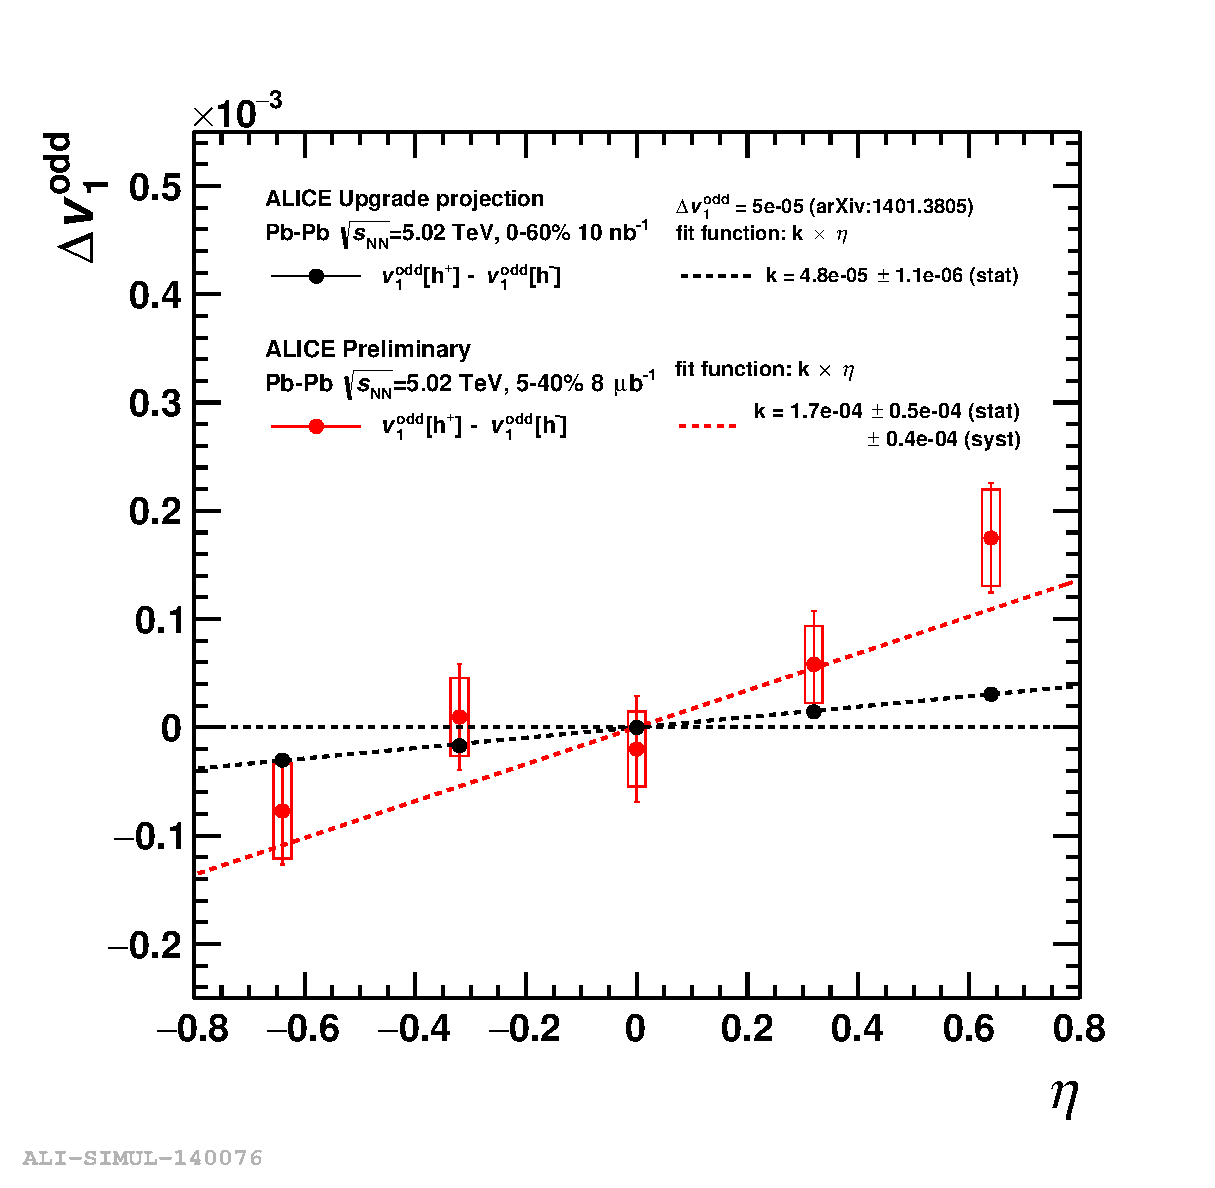
\includegraphics[width=0.8\textwidth]{figs/alice_projection_deltav1ch_stat8}
\caption{
}
\label{fig:alice_delta_v1}
\end{center}
\end{figure}


\begin{figure*}[!htb]
\begin{center}
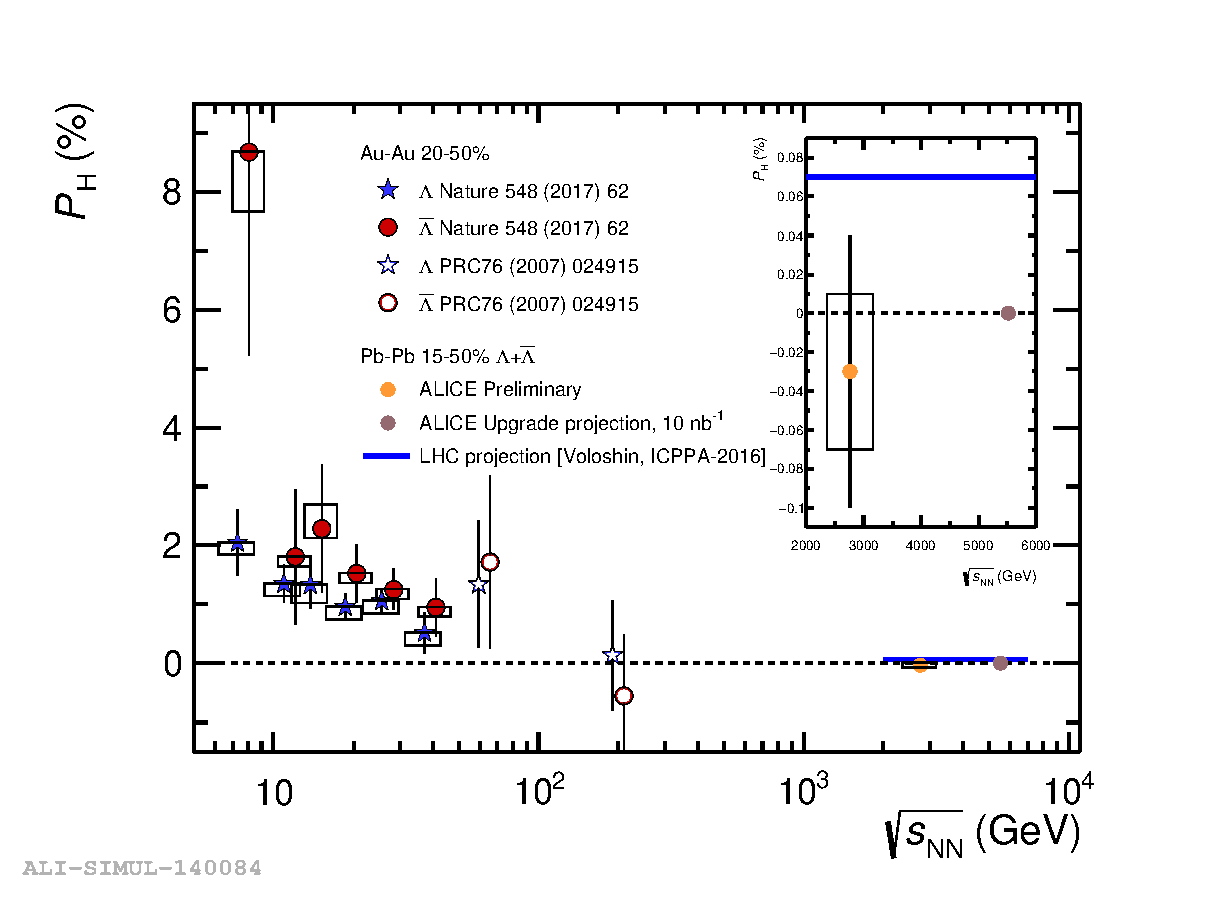
\includegraphics[width=0.8\textwidth]{figs/alice_projection_lambda}
\caption{Global polarization of $\Lambda$ and $\bar{\Lambda}$ as a function of the collision energy $\sqrt{s_{NN}}$ for semi-central heavy ion collisions. Open boxes
and vertical lines show systematic and statistical uncertainties,
respectively. Main panel: the data points for $\bar{\Lambda}$ are slightly horizontally shifted for visibility. Inner panel: the LHC energy domain is shown more detailed.
}
\label{fig:alice_lambda}
\end{center}
\end{figure*}

Fig. \ref{fig:alice_lambda} presents the energy dependence of the global polarization of $\Lambda$ and $\bar{\Lambda}$ for the semi-central heavy ion collisions. The RHIC results show the decrease of polarization at higher $\sqrt{s_{NN}}$. But $\Lambda$ and $\bar{\Lambda}$ demonstrate the finite global polarizations even at highest RHIC energy $\sqrt{s_{NN}}=200$ GeV \cite{PRC-98-014910-2018}. The preliminary ALICE data point at $\sqrt{s_{NN}}=2.76$ TeV is close in magnitude with results at $\sqrt{s_{NN}}=200$ GeV. But the ALICE upgrade projection at twice large collision energy corresponds to the zero polarization with very high precision. Therefore the study of global polarization of $\Lambda$ and $\bar{\Lambda}$ within HL--LHC project allows the unambiguous conclusion with regard of the values of this physics quantity in TeV-energy domain.    